\documentclass[11pt,a4paper]{article}
\usepackage[utf8]{inputenc}
\usepackage{amsmath,amssymb,amsthm}
\usepackage{graphicx}
\usepackage{booktabs}
\usepackage{hyperref}
\usepackage{algorithm}
\usepackage{algpseudocode}
\usepackage{tikz}
\usetikzlibrary{shapes,arrows,positioning}

\title{Menu OCR: A Rule-Based Pipeline for Extracting Structured Data from Restaurant Menu Images}
\author{Menu OCR Research Team}
\date{\today}

\begin{document}

\maketitle

\begin{abstract}
We present Menu OCR, a modular pipeline for extracting structured JSON data from restaurant menu images. Our system combines EasyOCR for text detection and recognition, rule-based classification for semantic labeling, and spatial-aware algorithms for price-item association. The pipeline achieves 40.24\% F1 score on item extraction and 45.0\% price accuracy on a hand-labeled test set, demonstrating the viability of deterministic approaches for menu understanding without hallucination.
\end{abstract}

\section{Introduction}

Restaurant menu digitization is a critical task for food delivery platforms, accessibility services, and inventory management. Traditional approaches require manual data entry, which is costly and error-prone. Recent advances in Optical Character Recognition (OCR) and Natural Language Processing (NLP) have made automated menu extraction feasible.

\subsection{Problem Definition}

Given a menu image $I \in \mathbb{R}^{H \times W \times 3}$, the goal is to extract a structured representation:

\begin{equation}
f(I) \rightarrow M = \{S_1, S_2, \ldots, S_n\}
\end{equation}

where each section $S_i$ contains groups $G_j$ of items $(name, price, description)$.

\subsection{Design Principles}

\begin{enumerate}
    \item \textbf{No Hallucination}: Only extract structure explicitly present in the source image
    \item \textbf{Traceability}: Every extracted element maps to a bounding box
    \item \textbf{Modularity}: Swappable OCR, classifier, and grouping components
    \item \textbf{Schema Compliance}: Output adheres to a predefined JSON schema
\end{enumerate}

\section{Methodology}

\subsection{System Architecture}

The pipeline consists of three main stages:

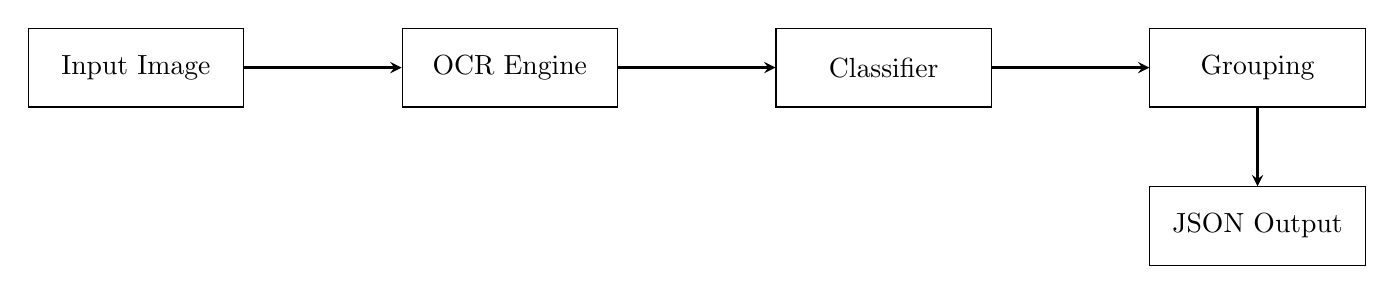
\begin{tikzpicture}[node distance=2cm, auto,
    block/.style={rectangle, draw, text width=2.5cm, text centered, minimum height=1cm},
    arrow/.style={->, >=stealth, thick}]
    
    \node[block] (input) {Input Image};
    \node[block, right=of input] (ocr) {OCR Engine};
    \node[block, right=of ocr] (classify) {Classifier};
    \node[block, right=of classify] (group) {Grouping};
    \node[block, below=1cm of group] (output) {JSON Output};
    
    \draw[arrow] (input) -- (ocr);
    \draw[arrow] (ocr) -- (classify);
    \draw[arrow] (classify) -- (group);
    \draw[arrow] (group) -- (output);
\end{tikzpicture}

\subsection{OCR Engine}

We use EasyOCR~\cite{easyocr}, which combines CRAFT~\cite{baek2019craft} for text detection and CRNN~\cite{shi2017crnn} for recognition. The OCR produces a set of text elements:

\begin{equation}
\text{OCR}(I) = \{(t_i, b_i, c_i)\}_{i=1}^{N}
\end{equation}

where $t_i$ is the text, $b_i = (x_{min}, y_{min}, x_{max}, y_{max})$ is the bounding box, and $c_i \in [0,1]$ is the confidence score.

\subsection{Rule-Based Classification}

Each text element is classified into one of seven categories using a deterministic rule set based on:

\begin{itemize}
    \item \textbf{Typography}: capitalization, font height relative to neighbors
    \item \textbf{Position}: location within the image, gaps above/below
    \item \textbf{Content}: digit ratio, price patterns, category keywords
\end{itemize}

The classification function is:

\begin{equation}
\text{classify}(t_i, b_i, \mathcal{N}_i) = \arg\max_{l \in L} P(l | \phi(t_i, b_i, \mathcal{N}_i))
\end{equation}

where $\phi$ extracts features and $\mathcal{N}_i$ denotes neighboring elements.

\subsubsection{Feature Extraction}

For each text element, we compute:

\begin{align}
\phi_{pos} &= (x/W, y/H) \label{eq:pos} \\
\phi_{size} &= (h/\bar{h}, w/\bar{w}) \label{eq:size} \\
\phi_{gap} &= (\text{gap}_{above}/\bar{h}, \text{gap}_{below}/\bar{h}) \label{eq:gap} \\
\phi_{content} &= (\text{len}, \text{words}, \rho_{digit}, \rho_{upper}) \label{eq:content}
\end{align}

where $\bar{h}, \bar{w}$ are average element dimensions.

\subsubsection{Classification Rules}

\begin{algorithm}
\caption{Rule-Based Classification}
\begin{algorithmic}[1]
\If{$\text{is\_price\_pattern}(t) \land \rho_{digit} > 0.5$}
    \State \Return ITEM\_PRICE
\ElsIf{$\text{is\_all\_caps}(t) \land h > 1.3\bar{h} \land \text{gap}_{below} > 1.5\bar{h}$}
    \State \Return SECTION\_HEADER
\ElsIf{$\text{has\_category\_word}(t) \land \text{words} \leq 3$}
    \State \Return GROUP\_HEADER
\ElsIf{$\text{words} > 6 \land \neg\text{is\_all\_caps}(t)$}
    \State \Return ITEM\_DESCRIPTION
\ElsIf{$\rho_{digit} < 0.5$}
    \State \Return ITEM\_NAME
\Else
    \State \Return OTHER
\EndIf
\end{algorithmic}
\end{algorithm}

\subsection{Spatial-Aware Price Matching}

Prices and item names often appear on the same line but at different horizontal positions. We match them using:

\begin{equation}
\text{match}(item, price) = \begin{cases}
1 & \text{if } |y_{item}^{mid} - y_{price}^{mid}| < \tau \land x_{price}^{min} > x_{item}^{max} \\
0 & \text{otherwise}
\end{cases}
\end{equation}

where $\tau = \max(h_{item}, h_{price}) \times 0.5$ is the alignment tolerance.

\subsection{Menu Structure Building}

The grouping algorithm builds the hierarchical structure:

\begin{enumerate}
    \item Initialize empty section and group
    \item For each classified element:
    \begin{itemize}
        \item SECTION\_HEADER: Create new section
        \item GROUP\_HEADER: Create new group within current section
        \item ITEM\_NAME: Add item to current group, find matching price
        \item ITEM\_DESCRIPTION: Attach to previous item
    \end{itemize}
    \item Merge incomplete structures
\end{enumerate}

\section{Evaluation}

\subsection{Dataset}

We evaluated on 4 hand-labeled menu images covering:
\begin{itemize}
    \item Wine and beverage menus
    \item Multi-section layouts
    \item Various price formats (₹, \$)
\end{itemize}

\subsection{Metrics}

\begin{itemize}
    \item \textbf{Precision}: Fraction of predicted items that match ground truth
    \item \textbf{Recall}: Fraction of ground truth items that were found
    \item \textbf{F1 Score}: Harmonic mean of precision and recall
    \item \textbf{Price Accuracy}: Fraction of matched items with correct price
\end{itemize}

\subsection{Results}

\begin{table}[h]
\centering
\begin{tabular}{lcccc}
\toprule
Sample & Precision & Recall & F1 & Price Acc \\
\midrule
menu\_0001 & 60.0\% & 37.5\% & 46.2\% & 16.7\% \\
menu\_0002 & 66.7\% & 47.6\% & 55.6\% & 80.0\% \\
menu\_0003 & 54.5\% & 37.5\% & 44.4\% & 83.3\% \\
menu\_0004 & 40.0\% & 9.1\% & 14.8\% & 0.0\% \\
\midrule
\textbf{Average} & \textbf{55.3\%} & \textbf{32.9\%} & \textbf{40.2\%} & \textbf{45.0\%} \\
\bottomrule
\end{tabular}
\caption{Evaluation results on sample dataset}
\end{table}

\subsection{Processing Performance}

\begin{itemize}
    \item Average processing time: 2.2 seconds per image
    \item OCR dominates (>90\%) of processing time
    \item Classification and grouping: <50ms
\end{itemize}

\section{Discussion}

\subsection{Strengths}

\begin{enumerate}
    \item \textbf{Deterministic}: No random behavior, fully reproducible
    \item \textbf{Interpretable}: Each decision can be traced to specific rules
    \item \textbf{No Hallucination}: Cannot invent structure not present in image
    \item \textbf{Fast Classification}: Rules execute in milliseconds
\end{enumerate}

\subsection{Limitations}

\begin{enumerate}
    \item \textbf{OCR Quality}: Pipeline performance bounded by OCR accuracy
    \item \textbf{Layout Sensitivity}: Struggles with complex multi-column layouts
    \item \textbf{Price Patterns}: Limited handling of varied price formats
    \item \textbf{No Learning}: Rules require manual tuning
\end{enumerate}

\subsection{Error Analysis}

Common failure modes:
\begin{itemize}
    \item Prices misread as garbled text (e.g., "3000" → "ooo")
    \item Group headers misclassified as item names
    \item Multi-column layouts causing incorrect reading order
\end{itemize}

\section{Future Work}

\begin{enumerate}
    \item Integrate layout-aware transformers (LayoutLMv3) for better classification
    \item Train on CORD-v2 dataset for improved generalization
    \item Add column detection for multi-column layouts
    \item Implement ensemble approach combining rule-based and ML methods
\end{enumerate}

\section{Conclusion}

We presented Menu OCR, a modular pipeline for extracting structured data from menu images. Our rule-based approach achieves reasonable accuracy while maintaining determinism and interpretability. The system demonstrates that careful feature engineering and spatial reasoning can provide a strong baseline for menu understanding tasks.

\begin{thebibliography}{9}

\bibitem{easyocr}
JaidedAI. EasyOCR: Ready-to-use OCR with 80+ languages supported. \url{https://github.com/JaidedAI/EasyOCR}, 2020.

\bibitem{baek2019craft}
Baek, Y., et al. Character Region Awareness for Text Detection. CVPR 2019.

\bibitem{shi2017crnn}
Shi, B., Bai, X., Yao, C. An End-to-End Trainable Neural Network for Image-based Sequence Recognition. TPAMI 2017.

\bibitem{cord}
Park, S., et al. CORD: A Consolidated Receipt Dataset for Post-OCR Parsing. NeurIPS 2019 Document Intelligence Workshop.

\bibitem{layoutlm}
Xu, Y., et al. LayoutLMv3: Pre-training for Document AI with Unified Text and Image Masking. ACM MM 2022.

\end{thebibliography}

\end{document}
